\chapter{Other Factors}

\section{Example}

In the following example, the same anchor set is used in four different random networks.  Figure~\ref{fig:AS6good}, shows two cases where the localization is normal.  
The figure plots a line between the real and calculated location of each node, giving a visual representation of the error.  

In two cases, the network errors are somewhat normal.  However, the other two cases are obviously terrible, with mean error being above three times the radio range.  With just a casual glance, the 2 outlier cases are seen to be caused by a reflection component of the linear transformation.  
\begin{figure}
  \centering
	\subfloat[Network A]{\label{fig:AS6NetworkDiff7}
		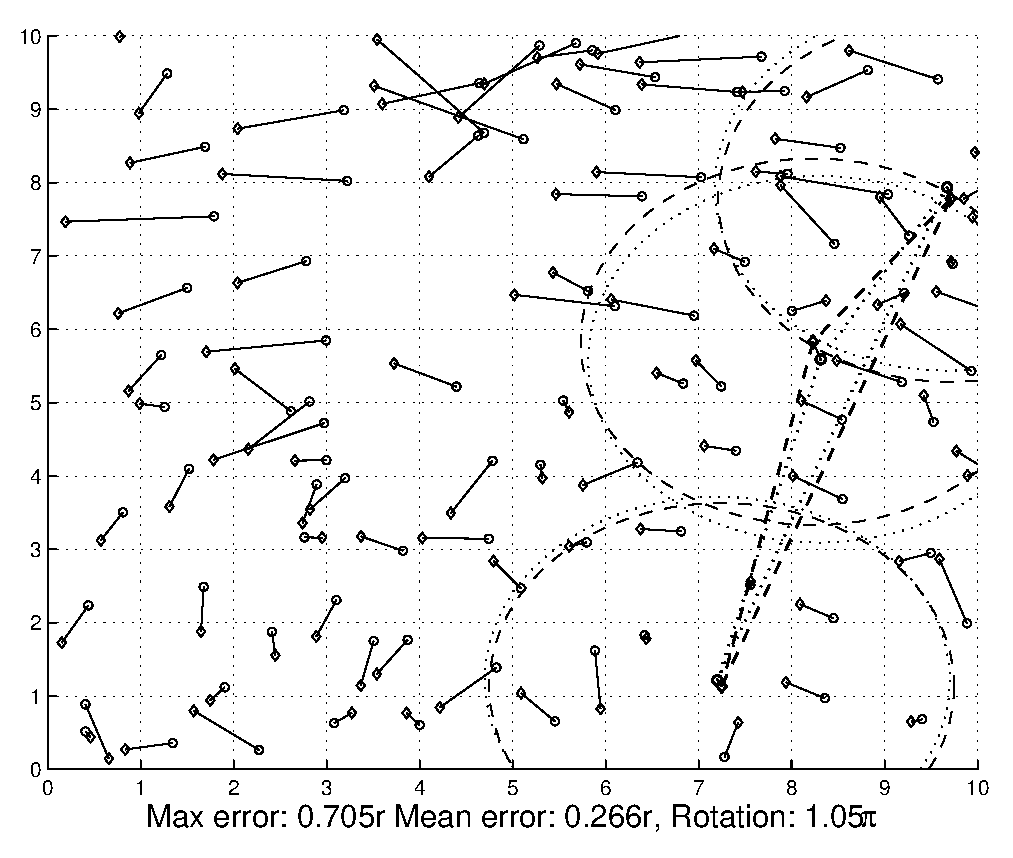
\includegraphics[width=0.5\textwidth]{outliers/AS6/AS6NetworkDiff7}}
	\subfloat[Network A]{\label{fig:AS6NetworkContour7}	
		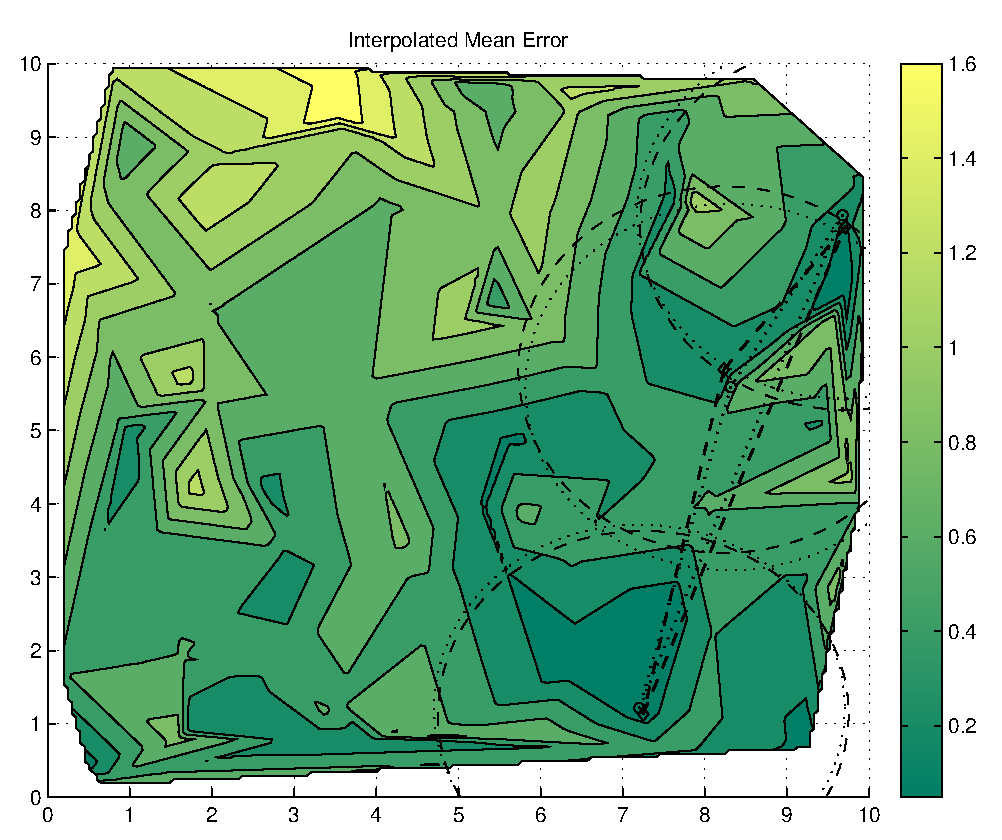
\includegraphics[width=0.5\textwidth]{outliers/AS6/AS6NetworkContour7}}
	\\
	\subfloat[Network B]{\label{fig:AS6NetworkDiff10}
		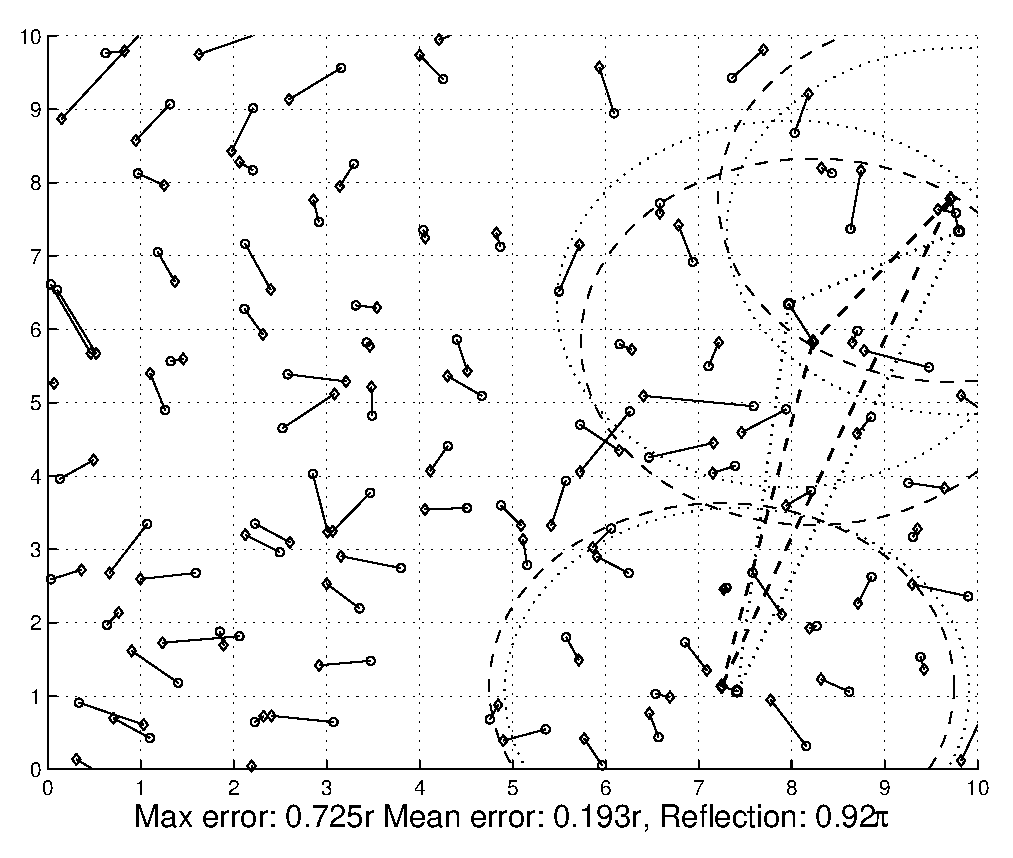
\includegraphics[width=0.5\textwidth]{outliers/AS6/AS6NetworkDiff10}}
	\subfloat[Network B]{\label{fig:AS6NetworkContour10}	
		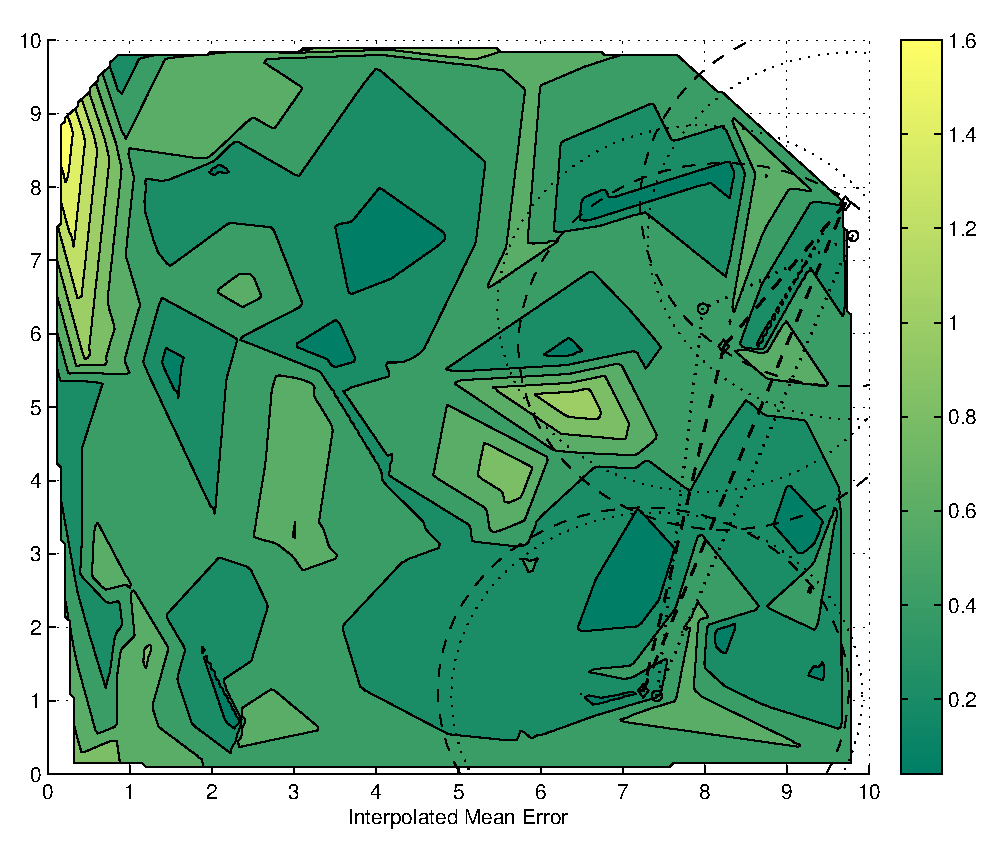
\includegraphics[width=0.5\textwidth]{outliers/AS6/AS6NetworkContour10}}
	\caption{2 different networks with the same anchor set}	
	\label{fig:AS6good}
\end{figure}
\begin{figure}
  \centering
	\subfloat[Network C]{\label{fig:AS6NetworkDiff9}
		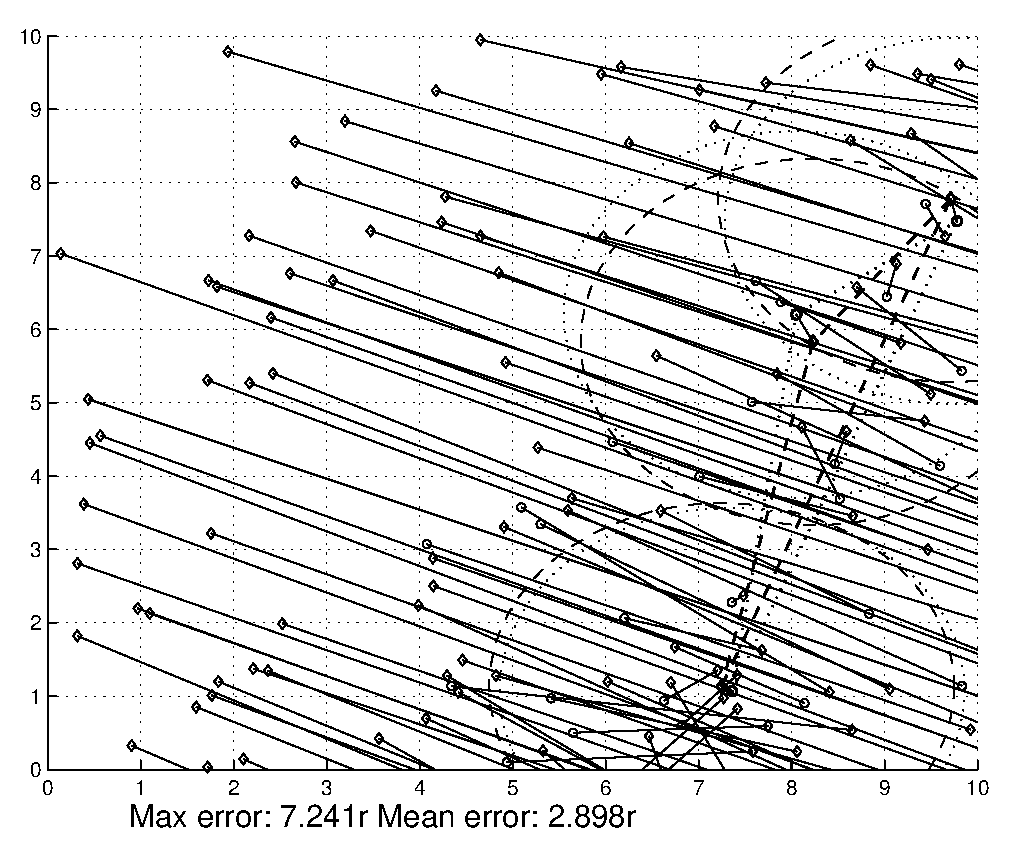
\includegraphics[width=0.5\textwidth]{outliers/AS6/AS6NetworkDiff9}}
	\subfloat[Network C]{\label{fig:AS6NetworkContour9}	
		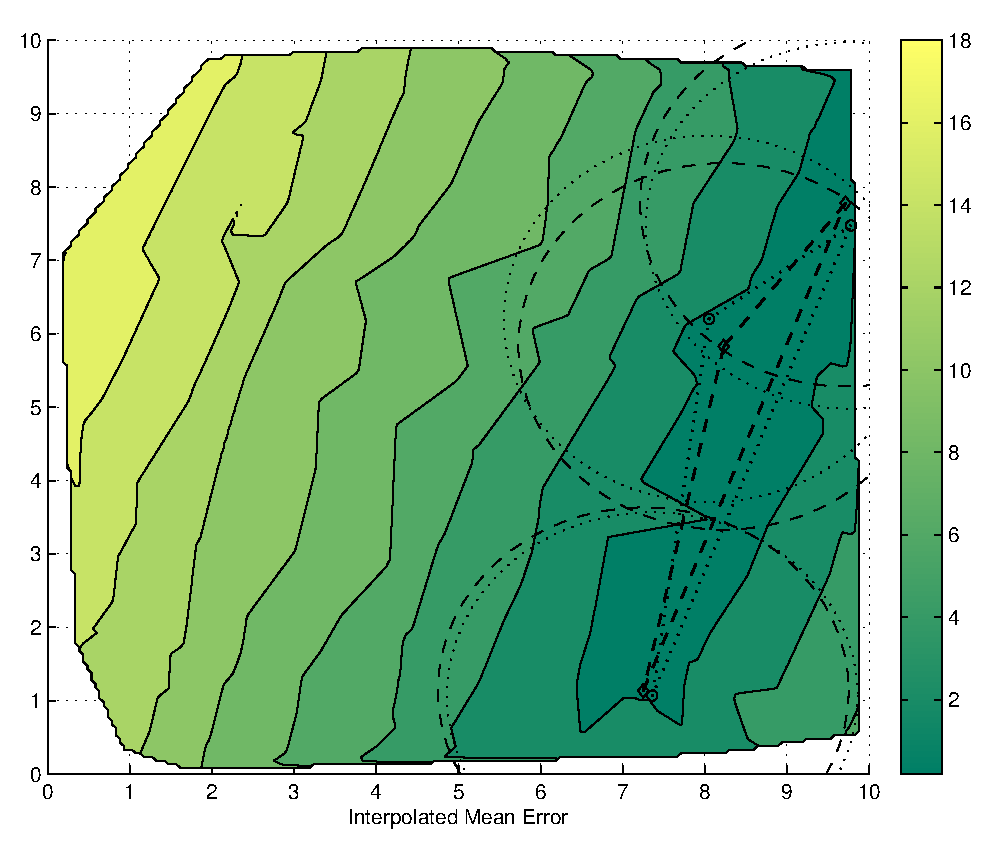
\includegraphics[width=0.5\textwidth]{outliers/AS6/AS6NetworkContour9}}
	\\
	\subfloat[Network D]{\label{AS6NetworkDiff8}
		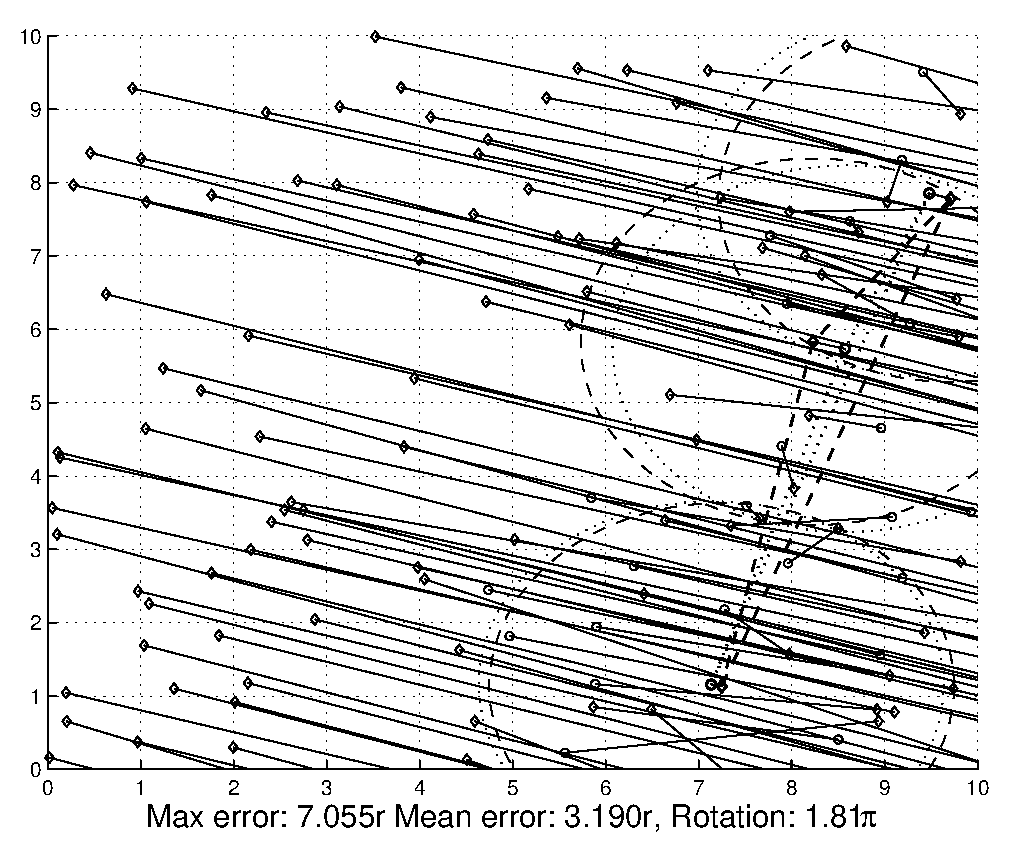
\includegraphics[width=0.5\textwidth]{outliers/AS6/AS6NetworkDiff8}}	
	\subfloat[Network D]{\label{fig:AS6NetworkContour8}	
		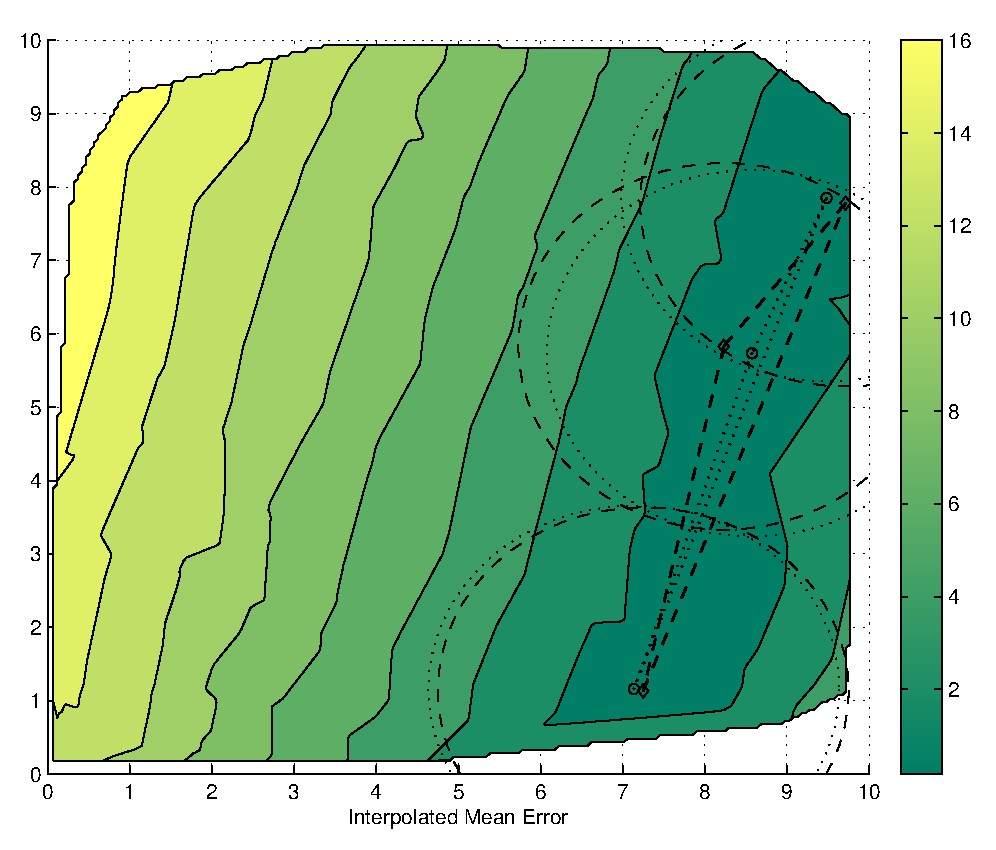
\includegraphics[width=0.5\textwidth]{outliers/AS6/AS6NetworkContour8}}
	\caption{2 more different networks with the same anchor set}	
	\label{fig:AS6bad}
\end{figure}
